%-----------------------------------------------------
% index key words
%-----------------------------------------------------
\index{geometry}
\index{dot product}
\index{orthogonal}

%-----------------------------------------------------
% name, leave blank
% title, if the exercise has a name i.e. Hilbert's matrix
% difficulty = n, where n is the number of stars
% origin = "\cite{ref}"
%-----------------------------------------------------
\begin{Exercise}[
name={},
title={}, 
difficulty=0,
origin={\cite{SM}}]
Use dot products to prove the Theorem of Thales: If $A$ and $B$ are endpoints of a diameter of a circle, and $C$ is any other point on the circle, then angle $\angle ACB$ is a right angle.
\begin{center}
    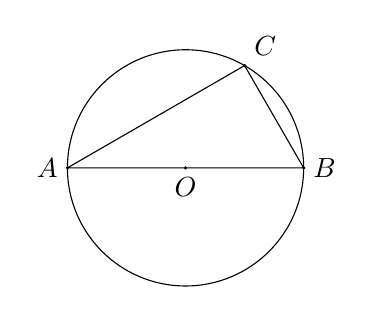
\begin{tikzpicture}[scale=0.5]
        \draw (0,0) circle [radius=3];
        \draw (-3,0) -- (3,0) -- (1.5,2.598) -- (-3,0);
        \node [below] at (0,0) {$O$};
        \node [left] at (-3,0) {$A$};
        \node [right] at (3,0) {$B$};
        \node [above right] at (1.5,2.598) {$C$};
        \draw[fill] (0,0) circle [radius=0.025];
        \draw[fill] (-3,0) circle [radius=0.025];
        \draw[fill] (3,0) circle [radius=0.025];
        \draw[fill] (1.5,2.598) circle [radius=0.025];
    \end{tikzpicture}
\end{center}

\end{Exercise}

\begin{Answer}
Hint: Let $O$ be the centre of the circle, and express everything in terms of $\overrightarrow{OA}$ and $\overrightarrow{OC}$.
\end{Answer}
